\documentclass[final,dissertation.tex]{subfiles}

%TC:group figure 0 0
%TC:macrocount \UoC 4
%TC:macrocount \mifare 1
%TC: macrocount \crypto 1
% chktex-file 29 (suppress "times might look prettier warning")

\begin{document}
  \chapter{Introduction}

  The \mifare{} Classic card is an NFC\footnote{Near Field Communication --- a set of communication protocols that enable two devices within close proximity of each other to communicate} based contactless smart-card with between \SI{1}{KB} and \SI{4}{KB} of protected memory. The cards are used for a wide range of applications, including micro-payments, ticketing, public transport and access control. The card is used within \UoC{} for access control to buildings as well as payment for meals at most colleges. To read or write data to the card an NFC reader must first authenticate with a secret key. Researchers have uncovered weaknesses in the card that allow an attacker to extract the secret keys and thus bypass the authentication. Given the range of applications the impact of this vulnerability is large.

  This project explores various countermeasures that an organisation can use to mitigate the risk of attack until they can move to a more secure card. The project consists of:
  \begin{itemize}
    \item A library for interacting with \mifare{} cards
    \item A simulation suite for simulating a network of readers and cards
    \item A library for reading and writing digitally signed data to \mifare{} cards
    \item A gossip protocol for distributing a list of revoked cards to offline readers (those without a network connection)
  \end{itemize}

  \section{Motivation}

  Since the vulnerabilities were made public in 2008, some organisations with large deployments of \mifare{} Classic cards have upgraded to cards without known exploits. Transport for London started replacing the \mifare{} Classic based Oyster cards with \mifare{} Desfire ones in 2010 to control fraud.

  Many organisations, including \UoC{}, have yet to upgrade and still rely on \mifare{} Classic cards for authentication and access control. More secure cards can't be issued until all the readers are upgraded to support them. For an organisation such as Cambridge, this is a fairly involved process which could take a long time. Cambridge consists of hundreds of suborganisations including departments and colleges, each of which have their own reader deployments.

  Existing research\cite{garcia2008dismantling}\cite{garcia2009wirelessly}\cite{courtois2008algebraic} has focussed on finding and exploiting weaknesses in the \mifare{} Classic card. It is common for these papers to conclude that the use of \mifare{} Classic cards should be deprecated in favour of more secure cards. These papers seldom consider the practical implications of upgrading and make no suggestions for how an organisation can protect themselves whilst upgrading.

  \section{Applicability to Other Cards}

  \emph{Defence in depth} is a security principle in which security measures are layered upon each other to provide redundancy when one security measure fails. Several of the countermeasures in this project can be used to enhance the security of other smart-cards and harden them against as yet unknown vulnerabilities.

  \section{Related Work}

  The security of \mifare{} Classic cards has been the subject of much academic interest. The proprietary encryption algorithm \crypto{} was partially reverse engineered by Nohl and Pl\"{o}tz in 2007~\cite{nohl:2007:ccc} by depackaging\footnote{Slicing the chip open, exposing the gates.} the chip and reverse engineering the gates as seen with a microscope. Garcia \emph{et.al.} built upon this and fully reverse engineered the algorithm in 2008\cite{garcia2008dismantling} by studying captured communication traces. Within the same paper, Garcia \emph{et.al.} proposed the first practical attack. The card manufacturer, NXP, attempted (and failed) to get a court injunction to prevent the publication of the research.

  Published research on digital signatures for NFC cards include a paper published on the NFC forum~\cite{rosati:2011:signatures} and a paper by Markus Kil\r{a}s~\cite{kilas:2009:signatures}.


  \section{Background}

  Over the past two decades, contactless smart-cards have become commonplace throughout the world. Amongst the most widely deployed are \mifare{} Classic cards, with over one billion produced.

  Communication between an NFC reader and a \mifare{} Classic card is protected by a protocol designed to provide mutual authentication. The authentication protocol uses a proprietary encryption algorithm called \crypto{}. Security researchers have discovered weaknesses that allow an attacker to extract the secret keys and thus bypass authentication.

  The goal of this project is not to completely ``secure'' \mifare{} Classic cards; the security of the cards is fundamentally broken. The goal is to provide countermeasures to allow an organisation to better protect themselves during the several years it may take to upgrade a large deployment of cards. The countermeasures described in this project significantly increase the complexity and resources required to successfully carry out an attack.

  \section{\mifare{} Classic Overview}

  The \mifare{} Classic card is one of several NFC cards manufactured and sold by NXP semiconductors (formerly part of Philips). The card conforms to parts one to three of the four part ISO 14443 Type A standard. The fourth part of the standard describes the transmission protocol between a card and a reader. NXP deviated from the standard to include their own proprietary encrypted communication protocol.

  The card is, in essence, a contactless memory card with read and write access protected by secret keys.

  \subsection{Logical Structure}
  The memory on the card is split into 16-byte blocks. These blocks are grouped into sectors, each sector having its own secret keys stored in its last block (the sector trailer). Blocks within a sector typically contain data that is logically connected as each block in the sector shares the same secret keys. For example, at \UoC{} one sector holds the CRSID\footnote{The Common Registration Scheme IDentifier is the identifier issued by the University Information Services to identify students and staff.} and student number whilst another sector holds data for door access to a particular college.

  There are two variants of the card, 1K and 4K. The 1K and 4K cards differ in both the size of memory and how it is divided into sectors (see Figure~\vref{fig:logical_structure}). The 1K card has 16 sectors, each of which has 4 blocks giving it a total memory of \SI{1024}{bytes}. The 4K card has 40 sectors, the first 32 sectors have 4 blocks and the last 8 have 16 blocks as shown in Figure~\vref{fig:logical_structure}, giving it a total memory of \SI{4096}{bytes}.

  \begin{figure}[h]
    \centering
    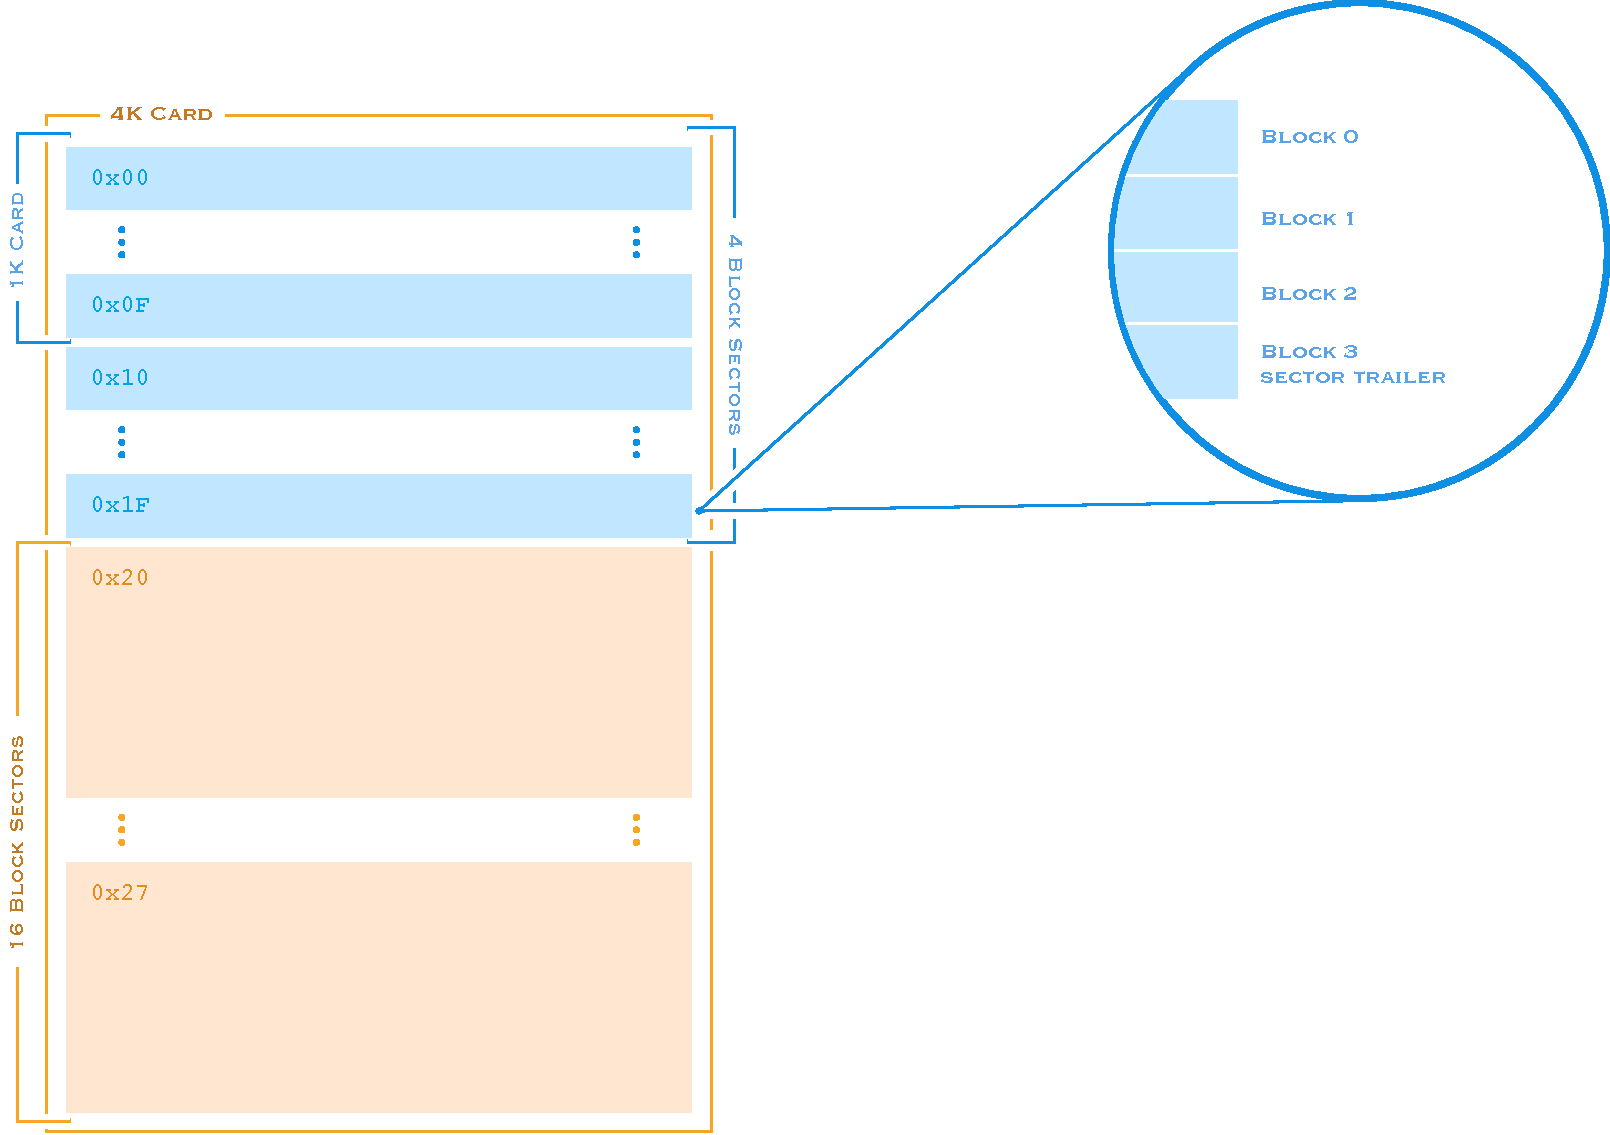
\includegraphics[width=\textwidth]{logical_structure.pdf}
    \caption{Logical Structure of Mifare Classic Cards}\label{fig:logical_structure}
  \end{figure}

  When NXP introduced the 4K card it was desirable to have no more than 40 sectors\footnote{The card uses a lookup table that allows a reader to lookup which sector contains certain data. To address more than 40 sectors the lookup table would have to occupy an additional sector itself.}. The non-uniform distribution of blocks to sectors in the 4K card was likely motivated by a desire to retain backwards compatibility whilst keeping within the limit of 40 sectors. By keeping the first 16 sectors of the 4K card the same as the 1K card, organisations are able to start issuing 4K cards without upgrading all their existing readers.

  \subsection{Blocks}
  All blocks except the last one in each sector are data blocks and can be used for storing data. The last block in each sector is the sector trailer, it contains the secret keys and access bits. The configuration of the access bits determines which operations can be performed by each key and whether a data block is a read/write block or a value block. The data layout and available operations vary between the two types of data block.

  \subsubsection{Read/Write Block}

  A generic read/write block contains 16 bytes of arbitrary data. The data is stored without parity bits and thus if data integrity is vital then parity bits should be added to the data itself. The configuration of the access bits determine which keys can perform each operation.

  \subsubsection{Value Block}

  Value blocks contain a signed 4-byte value and a 1-byte pointer to another block. The 4-byte value is stored three times, twice non-inverted and once inverted as shown in Figure~\vref{fig:value_block}. The 1-byte pointer is stored both inverted and non-inverted twice.

  \begin{figure}[h]
    \centering
    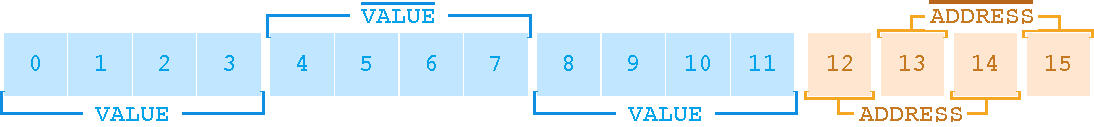
\includegraphics[width=0.7\textwidth]{value_block.pdf}
    \caption{Value Block}\label{fig:value_block}
  \end{figure}

  Value blocks are used in electronic wallet applications such as public transport ticketing systems where data integrity is very important. Storing the value three times provides strong protection against data corruption. This level of redundancy is warranted when a single flipped bit could have a large financial impact. The 1-byte address is used to store a pointer to a block containing a backup of the data.

  \subsubsection{Sector Trailer}
  The last block of each sector is the sector trailer, it contains:
  \begin{itemize}
    \item \bold{Access Bits} \\
      The access bits specify the operations that each key is allowed perform on each block of the sector.

    \item \bold{Secret Keys} \\
      Secret key A is always present, secret key B is optional. If the access bits are such that the memory typically occupied by key B is readable by key A then those bytes are treated as data and cannot be used to authenticate. When the sector trailer is read any secret keys are masked with zeros.

    \item \bold{User Data} \\
      The last byte of the access bits is unused, the \mifare{} Classic specification explicitly states that it is available for user data rather than being reserved for future use\cite{semiconductors2002mifare}.
  \end{itemize}

  The sector trailer is divided as shown in Figure~\vref{fig:sector_trailer}. The first six bytes contain key A. The next four contain the access bits, with the last byte ($9$) unused and available for user data. The remaining six bytes contain either key B or user data depending on whether the access bits allow it to be read.

  \begin{figure}[h]
    \centering
    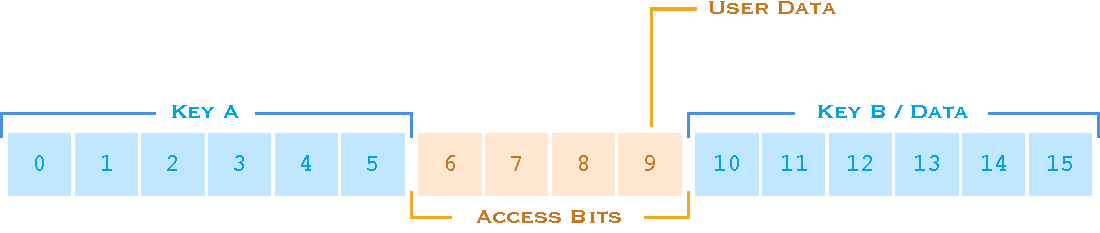
\includegraphics[width=0.7\textwidth]{sector_trailer.pdf}
    \caption{Sector Trailer}\label{fig:sector_trailer}
  \end{figure}

  \subsection{Memory Operations}

  There are six memory operations that can be performed on a block.

  \subsubsection{Read and Write}
  The read and write operations can be used wherever the access bits permit, irrespective of whether the block is a read/write block, value block or sector trailer. The operations read and write a block respectively. When reading the sector trailer zeros are returned in place of the keys.

  \subsubsection{Decrement, Increment, Restore and Transfer}
  These operations are only permitted on data blocks that are configured and formatted as value blocks. The decrement and increment operations decrement or increment a value block by a given argument and store the result in an internal register. The restore operation loads the value from a value block into the internal register\cite{semiconductors2002mifare}. The transfer operation transfers the value from the internal register into the value block\cite{semiconductors2002mifare}.
\end{document}
